\NeedsTeXFormat{LaTeX2e}
%\PassOptionsToClass{handout}{beamer}
\documentclass{beamer}
\usepackage{beamerPack}
\usepackage{pgfplots}
\usepackage[boxed,linesnumbered,ruled,vlined]{algorithm2e}
\usepackage{setspace}
\usepackage[02]{../lecture}
\subtitle{}
\usetikzlibrary{shapes.geometric,arrows,fit,matrix,positioning}
\tikzset{
  treenode/.style = {circle, draw=black, align=center, minimum size=1cm, anchor=center},
  subtree/.style = {regular polygon, regular polygon sides=3, draw=black, align=center, minimum height=0.5cm, minimum width=1cm, anchor=center}
}
\begin{document}

\begin{frame}[fragile]{}
\titlepage
\end{frame}

\section{time \& space complexity}		%%%%%%%%
\subsection{}

\begin{frame}[fragile]{アルゴリズムの性能(資源消費)の評価尺度}{}
\begin{block}{時間計算量}
実行に必要な時間。ハードウェア依存性をなくすため絶対時間ではなく命令実行回数が単位。
\end{block}
\begin{block}{空間計算量}
その計算を実行するために必要なメモリ量。ただしデータそのものは含めないことが多い。
Byte数よりも個数が単位。
\end{block}

\vfill
ただし定量的な比較が目的ではない。アルゴリズムAとBがN=1000の場合に何倍速度差があるかではなく、アルゴリズムAはNに対してどう変化するかを表現。
\begin{itemize}%\itemsep8pt
\item 

\end{itemize}

\end{frame}

\begin{frame}[fragile]{時間計算量}{}
\begin{block}{方針}
\begin{itemize}%\itemsep8pt
\item 命令(行)の実行回数で比較(実時間はハードウェア依存)
\item 最悪の場合を想定(平均は困難)
\item データの個数$N$に依存するため、$N$の関数として表現
\end{itemize}
\end{block}

\begin{columns}
\begin{column}{0.7\textwidth}
\scalebox{0.8}{
\begin{algorithm}[H]
%\TitleOfAlgo{線形探索}
%\SetAlgoRefName{lsearch}
\KwIn{v: \texttt{Vec<T>}}
\KwIn{条件 --- 引数を二分判定する関数}
\KwOut{発見または失敗}
\SetKwComment{Comment}{}{}
i = 0\;
\While{iが要素数より小さい} {
  \If{v[i]が条件を満たす}{
    \Return{発見}
  }
  i += 1\;
}
\Return{失敗}\;
\caption{線形探索}
\end{algorithm}
}
\end{column}
\begin{column}{0.25\textwidth}

\begin{itemize}%\itemsep8pt
\item L1: 1
\item L2: 最悪N
\item L3: 最悪N
\item L4: 最悪1
\item L5: 最悪N
\item L6: 最悪1
\end{itemize}
\end{column}
\end{columns}
\end{frame}

\begin{frame}[fragile]{計算の簡略化:Nに対する変化にのみ注目}{}
\begin{itemize}%\itemsep8pt
\item おそらく条件検査L3が1番時間が掛かる
\item L3とL5の実行回数はほぼ一緒
\item L3のif文を数えることに帰着させる(係数の差程度)
\end{itemize}

\vfill
\begin{columns}[T]
\begin{column}{0.6\textwidth}
\scalebox{0.7}{
\setcounter{algocf}{0}
\begin{algorithm}[H]
\KwIn{v: \texttt{Vec<T>}}
\KwIn{条件}
\KwOut{発見または失敗}
\SetKwComment{Comment}{}{}
i = 0\;
\While{iが要素数より小さい} {
  \If{v[i]が条件を満たす}{
    \Return{発見}
  }
  i += 1\;
}
\Return{失敗}\;
\caption[page]{線形探索}
\end{algorithm}
}
\end{column}
\begin{column}{0.5\textwidth}
L3の実行回数はL2の実行回数。

\begin{block}{}
線形探索の時間計算量は$N$。
\end{block}

{\fontsize{8}{8}\selectfont 比例関係であることがわかった。}

\medskip
計算上では。
\end{column}
\end{columns}
\end{frame}

\begin{frame}[fragile]{参考1:Criterionで実測}{}
\begin{center}
\begin{tikzpicture}
\node at (0,0) {\pgfimage[width=0.8\pagewidth]{criterion1.png}};
\end{tikzpicture}
\end{center}

\begin{spacing}{0.7}
\fontsize{7}{7}\selectfont
N=1M個に対し経過時間$100 \mu 秒 = 0.1 m秒$。1GHzのCPU(パイプライン無視して1M命令/1m秒)ならその間に0.1M命令。4GHzまでオーバーブーストかつパイプラインで最低4命令同時実行でようやく桁がギリギリ合うくらいなのだが。。。
\end{spacing}
\end{frame}

\begin{frame}[fragile]{参考2:対応する機械語\href{https://godbolt.org}{\beamergotobutton{Compiler Explore}}}{}
\begin{tikzpicture}[overlay, xshift=0.5\textwidth]
\node at (0,-1) {\pgfimage[width=1.0\pagewidth]{assembled.png}};
\end{tikzpicture}
\end{frame}

\begin{frame}[fragile]{理論値が示すもの}{}
% \begin{tikzpicture}[overlay, xshift=0.6\textwidth, yshift=-0.6\textheight]
% \draw[help lines, thin, step=0.5, color=gray] (0,0) grid (2,2);
% \draw (0, 0) .. controls (0.5, 0.7) and (1.5,1.5) .. (2, 1.5);
% \draw (0, 0) .. controls (0.5, 0.4) and (1.5,1) .. (2, 2);
% \end{tikzpicture}

\begin{center}
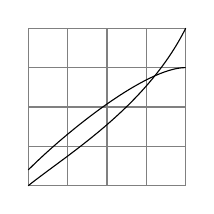
\begin{tikzpicture}
\draw[help lines, thin, step=0.5, color=gray] (0,0) grid (2,2);
\draw (0, 0.2) .. controls (0.5, 0.7) and (1.5,1.5) .. (2, 1.5);
\draw (0, 0) .. controls (0.5, 0.4) and (1.5,1) .. (2, 2);
\end{tikzpicture}
\end{center}



\begin{itemize}\itemsep8pt
\item 「スケーラビリティ」
\begin{itemize}%\itemsep8pt
\item 全ての$N$に対する予言、ではない
\item 特定の$N$でのよしあし、ではない
\item 誤差の無視、ではない(「無視できる」だけ)
\end{itemize}
\item 極限は無限大に飛ばす操作なのでこの文脈では不適切
\end{itemize}
\end{frame}

\section{$O$-notation}		%%%%%%%%
\subsection{}

\begin{frame}[fragile]{$O$-記法}{}
実数値関数 $f(x)$ と $g(x)$ に対し、

\begin{align*}
\exists x_{0}, \exists M > 0,  \forall x > x_{0} : |f(x)| < M | g(x) |
\end{align*}
が成立するとき(またその時に限り)、

\begin{align*}
f(x) &= O(g(x))
\end{align*}
\end{frame}

\begin{frame}[fragile]{足掛かり1}{}

実行時間(命令回数)の測定結果を表す$f(x)$と何か数学的な関数$g(x)$に対し、

\begin{align*}
適当に x_{0}と係数M > 0を決めたら & \\
x_{0}以上の範囲では& fより M g が大きい.
\end{align*}
ことがわかったら、

\begin{align*}
f(x) &= O(g(x))
\end{align*}
と書こう。
\end{frame}

\begin{frame}[fragile]{足掛かり2}{}

\begin{itemize}\itemsep20pt
\item 「データ数$100$まで理論通りになりません」あるいは「データ数$100$で実験したら線形探索の方が速かったです」
\begin{itemize}
\item $x_{0} = 100$とすれば騒ぐことではないな
\end{itemize}
\item 「こっちのPCでは実験結果は$O(N^2)$、あっちのだと$O(2.4N^2)$になりました」
\begin{itemize}
\item $M=2.4$とおいたらどちらも同じなのに
\item p4でL1, L5などを無視したのは$O$-記法で消えてしまうから
\end{itemize}
\item なぜ絶対値
\begin{itemize}%\itemsep8pt
\item 時間測定に限定させない一般化(波のenvelop関数)
\end{itemize}
\end{itemize}
\end{frame}

\begin{frame}[fragile]{$O$-記法の解釈と例}{}

$f(x) = O(g(x))$なら$f$は$g$で上から抑えられる、すなわち上限

\begin{align*}
1.5 x & = O(x) \\
\sum_{1}^{n=N} n & = O(N^2) \\
0.001x^2 + 2000000x & = O(x^2 + x) \\
         & = O(x^2) \\
\end{align*}

\vfill
以下は(ほぼ)間違い。近似関係ではなく等値関係。
\begin{align*}
2.14x^3 \approx O(x^3), &\quad 2.14x^3 \le O(x^3)
\end{align*}
\end{frame}

\begin{frame}[fragile]{$\Omega(-)$, $\Theta(-)$}{}
\begin{align*}
\exists x_{0}, \exists M > 0,  \forall x > x_{0} : |f(x)| > M | g(x) |
\end{align*}
が成立するとき(またその時に限り)、

\begin{align*}
f(x) &= \Omega(g(x)).
\end{align*}

\vfill
さらに
\begin{align*}
f(x) = O(g(x)) && f(x) = \Omega(g(x))
\end{align*}
が成立するとき(またその時に限り)、

\begin{align*}
f(x) &= \Theta(g(x))
\end{align*}
\end{frame}

\section{order of search}		%%%%%%%%
\subsection{}

\begin{frame}[fragile]{線形探索の計算量}{}
「線形探索の実行時間は$N$」から、

\begin{block}{線形探索の計算量}
\begin{itemize}\itemsep8pt
\item 線形探索の時間計算量は$O(N)$\footnotemark
\item 線形探索の空間計算量は$O(1)$\footnotemark
\end{itemize}
\end{block}

[1]{読み方は色々:オー、ビッグオー、オーダーなど}

[2]{(再帰しない関数で)ローカル変数を$X$個定義しても$X = O(1)$}

\footnotetext[1]{読み方色々:オー、ビッグオー、オーダーなど}
\footnotetext[2]{(再帰しない関数で)ローカル変数を$X$個定義しても$X = O(1)$}
\end{frame}

\begin{frame}[fragile]{二分探索の計算量}{}
\scalebox{0.7}{
\begin{algorithm}[H]
\SetKwComment{Comment}{}{}
\BlankLine
i = 0; j = z.len() - 1\Comment*{\sl\small\color[gray]{0.5}探索範囲}
\While{i <= j} {
  \If{ v[(i + j) / 2]が等しい}{
    \Return{発見}
  }
  \eIf{v[(i + j) / 2]が小さい}{
    i = (i + j) / 2 + 1\Comment*{\sl\small\color[gray]{0.5}探索範囲の左半分を破棄}
  }{
    j = (i + j) / 2 - 1\Comment*{\sl\small\color[gray]{0.5}探索範囲の右半分を破棄}
  }
}
\Return{失敗}\;
\caption[page]{二分探索}
\end{algorithm}
}

\vfill

\begin{itemize}%\itemsep8pt
\item データの大きさが$N$の場合の繰り返し回数: $\log_{2}(N)$
\item 各繰り返しの中で実行する条件比較は2回=$O(1)$回
\item $1回あたりO(1) \times 繰り返し回数O(\log(N)) = 計 O(\log(N))$
\item ローカル変数が二つ= $O(1)$
\end{itemize}
\end{frame}

\begin{frame}[fragile]{$\log_2(N)$の理由}{}

{%\fontsize{9}{10}\selectfont
\begin{tabular}[h]{|c|r| r |}
\CH $N$ & 範囲の(最悪)変化 & 繰返し回数 \\
\CL $1$ & $1$ & $1$ \\
\CL $3$ & $3 \to 1$ & $2$ \\
\CL $7$ & $7\to3\to1$ & $3$ \\
\CL $15$ & $15\to7\to3\to1$ & $4$ \\
\CL $2^x - 1$ & $2^{x} -1 \to 2^{x-1} - 1 \to \cdots \to 2^1 - 1$ & $x$ \\
\CL $N$ & -- & $\log_2(N)$ \\
\end{tabular}
}

\medskip
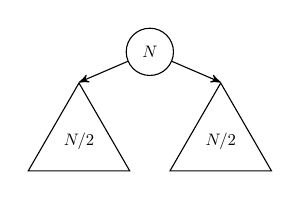
\begin{tikzpicture}[->,>=stealth',level/.style={sibling distance = 3.0cm/#1, level distance = 1.9cm},scale=0.6, transform shape]
\node [treenode] {$N$}
    child[child anchor=north] { node [subtree] {$N/2$} }
    child[child anchor=north] { node [subtree] {$N/2$} }
    ;
\end{tikzpicture}

\end{frame}

\begin{frame}[fragile]{探索の計算量まとめ}{}

{%\fontsize{9}{10}\selectfont
\begin{tabular}[h]{|c|r|r|r|}
\CH アルゴリズム & (最悪)時間計算量 & 最良時間-- & 空間-- \\
\CL 線形探索 & $O(N)$ & $O(1)$ & $O(1)$ \\
\CL 二分探索 & $O(\log(N))$ & $O(1)$ & $O(1)$ \\
\end{tabular}
}

\vfill
{\fontsize{8}{8}\selectfont
$O$-記法を使ったことで係数が消えているので、直接の速度比較はできない。
それぞれが$N$に対してどう変化するのかを言うもの。

逆に$O$-記法での比較が最終目的なら、各行の実行回数を全て数え上げたりしなくてよい。
}
\end{frame}

\begin{frame}[fragile]{Criterionで実測2}{}
\begin{center}
\begin{tikzpicture}
\node at (0,0) {\pgfimage[width=0.8\pagewidth]{criterion2.png}};
\end{tikzpicture}
\end{center}

\vfill
両対数グラフであることに注意
\end{frame}

\begin{frame}[fragile]{別解}{再帰$\to$帰納法$\to$数列の一般項}
\begin{columns}
\begin{column}{0.5\textwidth}
\begin{codeof}{language=Rust}{再帰版lsearch}
fn lsearch(長さ\@N@,c) {
  c();
  lsearch(長さ\@N-1@, c);
}
\end{codeof}
\begin{align*}
T(n) = & O(1) \\
& + T(n-1)\\
= & n O(1) \\
T(N) = & O(N)
\end{align*}

\end{column}
\begin{column}{0.5\textwidth}
\begin{codeof}{language=Rust}{再帰版bsearch}
fn bsearch(長さ\@$N$@, c) {
  c();
  bsearch(長さ\@$N/2$@, c);
}
\end{codeof}
\begin{align*}
T(n) = & O(1) \\
& + T(n/2)\\
= & O(1) O(\log(n)) \\
T(N) = & O(\log(N))
\end{align*}
\end{column}
\end{columns}
\end{frame}

\begin{frame}[fragile]{参考}{}

\begin{columns}[T]
\begin{column}{0.5\textwidth}
\begin{align*}
T(n) = & O(n) \\
& + T(n-1)\\
= & n + (n - 1) + \cdots + 1 \\
T(N) = & O(N^2)
\end{align*}
\end{column}

\begin{column}{0.5\textwidth}
\begin{align*}
T(n) = & O(n) \\
& + T(n/2) + T(n/2)\\
= & O(n) + 2T(n/2) \\
= & O\left(\frac{n}{1} + \frac{2n}{2} + \frac{4n}{4} + \cdots \right) \\
T(N) = & O(N\log(N))
\end{align*}
\end{column}
\end{columns}

\end{frame}

\begin{frame}[fragile]{より速い探索}{}
\begin{block}{ハッシュ表とハッシュ関数}
\begin{itemize}%\itemsep8pt
\item 時間計算量はほぼ$O(1)$
\item 空間計算量は$O(データの潜在的総数)$\footnotemark
\end{itemize}
\end{block}

\begin{block}{特定の検索に対する高速化(最大値検索)}
\href{https://ja.wikipedia.org/wiki/赤黒木}{\beamergotobutton{赤黒木}},
\href{https://ja.wikipedia.org/wiki/トライ_(データ構造)}{\beamergotobutton{トライ木}},
\href{https://ja.wikipedia.org/wiki/2-3-4木}{\beamergotobutton{2-3-4木}}などの木構造が適している
\end{block}

\begin{block}{並列探索}
固定の$M$台使用するなら$O(N/M) = O(N)$。
データの大きさに合わせて増加させるなら$O(N)$以下が可能。
\end{block}

[3]{正確には$O(|ハッシュ関数の値域|)$}

\footnotetext[3]{正確には$O(|ハッシュ関数の値域|)$}
\end{frame}

\end{document}
